% !TeX spellcheck = en_US

\chapter{Implementação do Sistema}

Um protótipo de uma Base de Dados de WhiteSpace (BDWS)
\abbrev{BDWS}{Bases de Dados de WhiteSpace}
foi implementado anteriormente por Marcelo Machado em seu trabalho de conclusão de curso~\cite{tccmarcelo}. Essa base é capaz de indicar a um US os canais livres no espectro de frequência, permitindo sua utilização. Para isso, a base possui informações sobre todos os UPs presentes. É passado como parâmetro de entrada a localização do US e a base retorna uma resposta com a lista de canais disponíveis para uso.

O espectro de frequência é extenso e utilizado para várias finalidades, como Transmissão de dados para satélites, rádio navegação e transmissão de TV. Atualmente, a base implementada possui apenas informações referentes ao espectro de transmissão de TV, que vai de 54 Mhz até 806Mhz~\cite{fccalloc} .

A base possui as informações referentes às antenas de televisão que operam na região do Estado do Rio de Janeiro. Esses dados foram obtidos da ANATEL~\cite{channelstable}. Certos dados oriundos da agência reguladora estão incompletos e inconsistentes, o que acarreta erros de cálculo na base. Torna-se necessária uma maior cooperação entre a agência reguladora com a base, para aumentar a confiabilidade das respostas às requisições dos USs.

\section{Cálculo dos Canais Disponíveis}

O servidor consulta o banco de dados e coleta as informações das antenas presentes no Estado do Rio de Janeiro. A partir de sua altura e potência, calcula-se o alcance máximo para cada antena, dependendo do modelo de propagação do sinal. O alcance máximo é definido como: "A distância máxima da base da antena que um dispositivo pode estar para receber o sinal transmitido por ela com uma relação sinal/ruído mínima. Assume-se que o dispositivo não sofre nenhuma interferência além de duas vezes ruído de fundo". Os dispositivos que possuírem uma distância menor que o raio da antena, receberão o sinal com qualidade suficiente. Já os dispositivos com distancia da antena maior que seu raio, estarão fora do alcance da mesma, podendo utilizar esse canal para transmissão de seus dados. Essa condição é necessária para que um US possa transmitir dados nessa frequência sem causar interferências.

Assumindo um Usuário Primário P com alcance \begin{math}p\end{math} e um Usuário Secundário S com alcance \begin{math}s\end{math}. Sendo D a distância entre P e S. O US S poderá transmitir dados utilizando o canal de P somente se:

\begin{align}
  \label{cantransmitdata} p + s > D
\end{align}

Os alcances \begin{math} p \end{math} e \begin{math} s \end{math} são obtidos através dos modelos de propagação implementados na base. Os modelos que foram implementados anteriormente são: 

\begin{itemize}
\item Free Space
\item Two Ray Ground
\item Log Distance
\end{itemize}

\subsubsection{Modelos de Propagação Implementados}

Cada modelo retorna um valor de atenuação, no qual a relação sinal/ruído se torna igual a 10dB. Esse modelo é aplicado tanto para o UP quanto para o US, e com isso, encontra-se a distância máxima do alcance de um dispositivo. Para isso, é necessário encontrar a relação sinal/ruído, definida:

\begin{align}
  \label{Sinr} SINR=\frac{P}{I+N}
\end{align}

Onde \textit{P} é a potência do sinal, \textit{I} é a interferência e \textit{N} é o ruído de fundo.

Como é assumido que a única interferência no ambiente será o ruído de fundo, tem-se então que:

\begin{align}
  \label{actSinr} SINR=\frac{P}{N}
\end{align}

O ruído de fundo, em Watts, é definido como:

\begin{align}
  \label{noise} Noise=kTB
\end{align}

Aonde \textit{k} é a constante de Boltzman, \textit{T} é a temperatura do ambiente e \textit{B} é a banda em hertz.

Assim, pelas equações~\ref{actSinr} e~\ref{noise} tem-se que a potência mínima do receptor é:

\begin{align}
  \label{minPot} P_r= SINR \cdot  kTB
\end{align}

O valor da relação sinal/ruído deve ser convertido para W de forma a facilitar os cálculos. Dessa forma:

\begin{align}
  \label{SinrW} 10= 10 log_{10} (SINR_W)
\end{align}

De modo que a potência do sinal emitido pela antena em seu alcance máximo será:

\begin{align}
  \label{minPotAnt} P_{a}= 10kTB
\end{align}

 No entanto, o dispositivo que utiliza o WS não pode interferir com os receptores da antena. Dessa forma, seu sinal deve ser atenuado até atingir o valor do ruído de fundo. Assim sendo, a relação sinal/ruído deve ser de 0dB. De modo que podemos determinar a potência no alcance máximo do dispositivo como sendo:

\begin{align}
  \label{minPotDev} P_{d}=  kTB
\end{align}

\subsubsection{Free Space}

O modelo de propagação Free Space assume que o transmissor e o receptor possuem um caminho em linha reta, sem obstáculos próximos que possam causar os fenômenos de difração ou interferência. Esse modelo raramente é utilizado exclusivamente, normalmente faz parte de um modelo maior, como o Longley-Rice. Por desconsiderar as irregularidades do solo e assumir que o meio é sem obstrução, os alcances acabam sendo muito maiores do que a realidade. O modelo é ilustrado na figura abaixo\ref{fig:freespaces}.

\begin{figure}[htb]
\centering
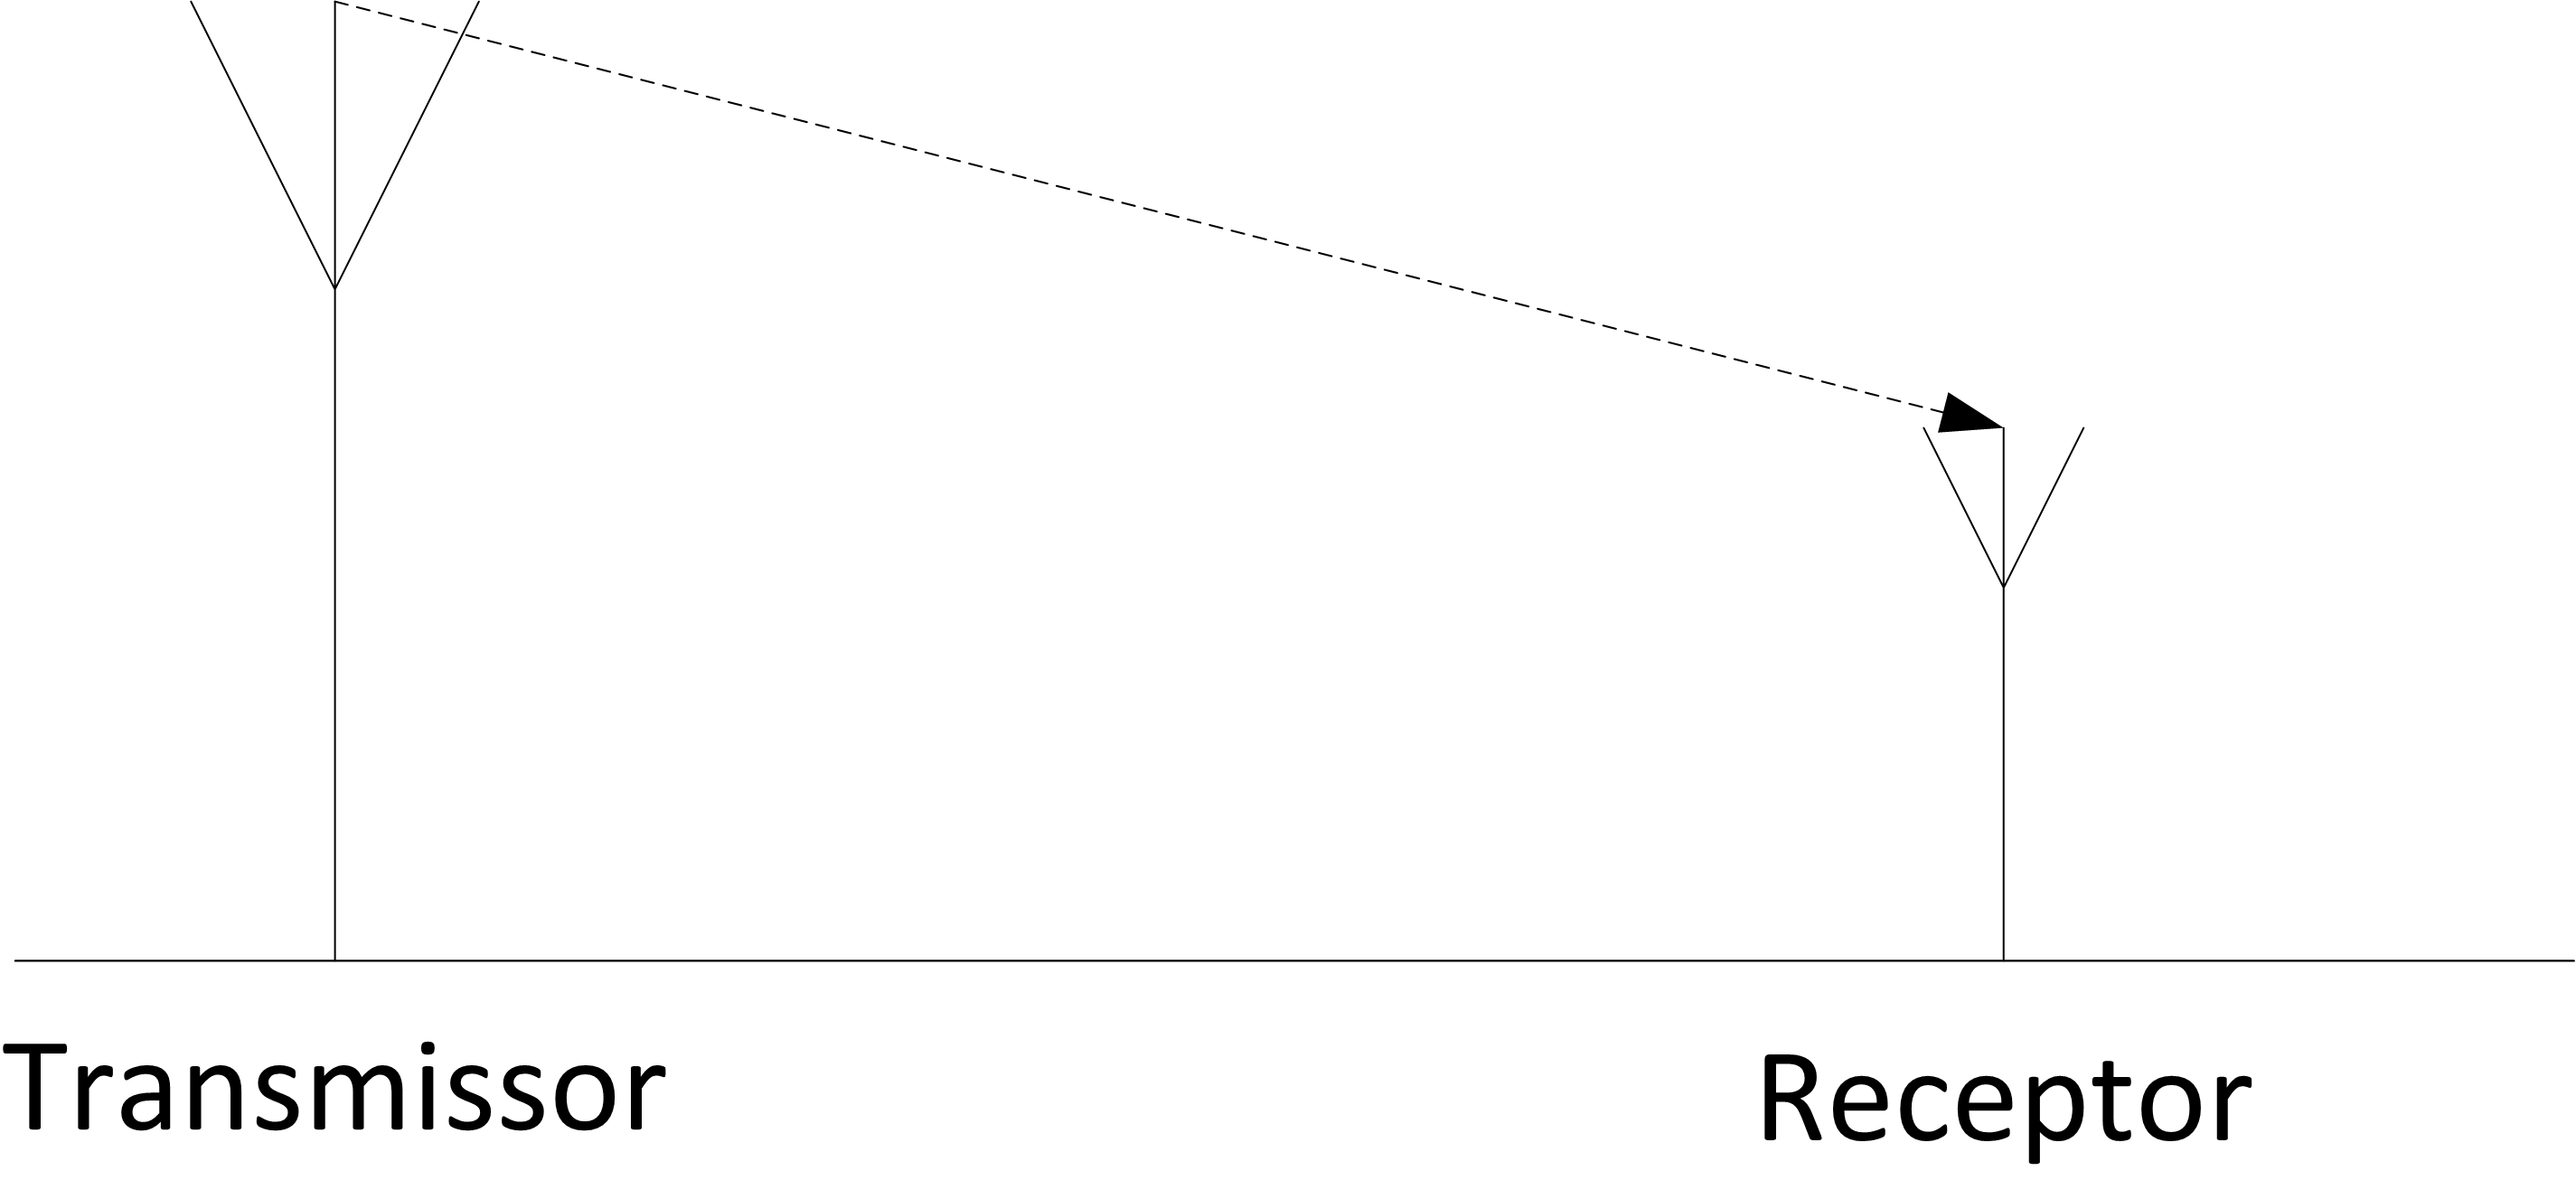
\includegraphics[width=0.8\textwidth]{figs/freespaces}
\caption[Modelo de propagação Free Space.]
{Modelo de propagação Free Space.}
\label{fig:freespaces}
\end{figure}

A potência recebida pelo receptor quando o transmissor se encontra a uma distância \textit{d} é definida~\cite{rapapport} como: 

\begin{align}
  \label{potfree} P_r(d) =\frac{ P_tG_tG_r\lambda^{2}}{(4\pi)^{2}d^{2}L}
\end{align}

\begin{math}G_t\end{math} e \begin{math}G_r\end{math} são os ganhos do transmissor e receptor respectivamente. Foi assumido que a potência indicada pela ANATEL é, na verdade, \begin{math}P_tG_t\end{math}, enquanto \begin{math}G_r\end{math} foi desconsiderado.

\begin{align}
  \label{ganho} G_r = 1
\end{align}

\textit{L} representa o fator de perda não relacionado ao modelo de propagação. L também foi desconsiderado.

\begin{align}
  \label{loss} L = 1
\end{align}

\begin{math}\lambda\end{math} é referente a frequência utilizada para transmissão, onde \textit{c} é a velocidade da luz em m/s e \textit{f} é a frequência utilizada em Hz.

\begin{align}
  \label{lambda}\lambda=\frac{c}{f}
\end{align}

Assim sendo, determina-se o alcance de uma antena no modelo de Free Space pelas equações~\ref{potfree} e~\ref{minPotAnt}:

\begin{align}
  \label{dFreeAnt} d_1 = \sqrt{\frac{P_t\lambda^{2}}{10kTBL(4\pi)^{2}}}
\end{align}

De maneira análoga, o alcance de um US pode ser determinado pelas equações~\ref{potfree} e~\ref{minPotDev}:

\begin{align}
  \label{dFreeDev} d_2 = \sqrt{\frac{P_t\lambda^{2}}{kTBL(4\pi)^{2}}}
\end{align}

\subsubsection{Two Ray Ground}

\begin{figure}[htb]
\centering
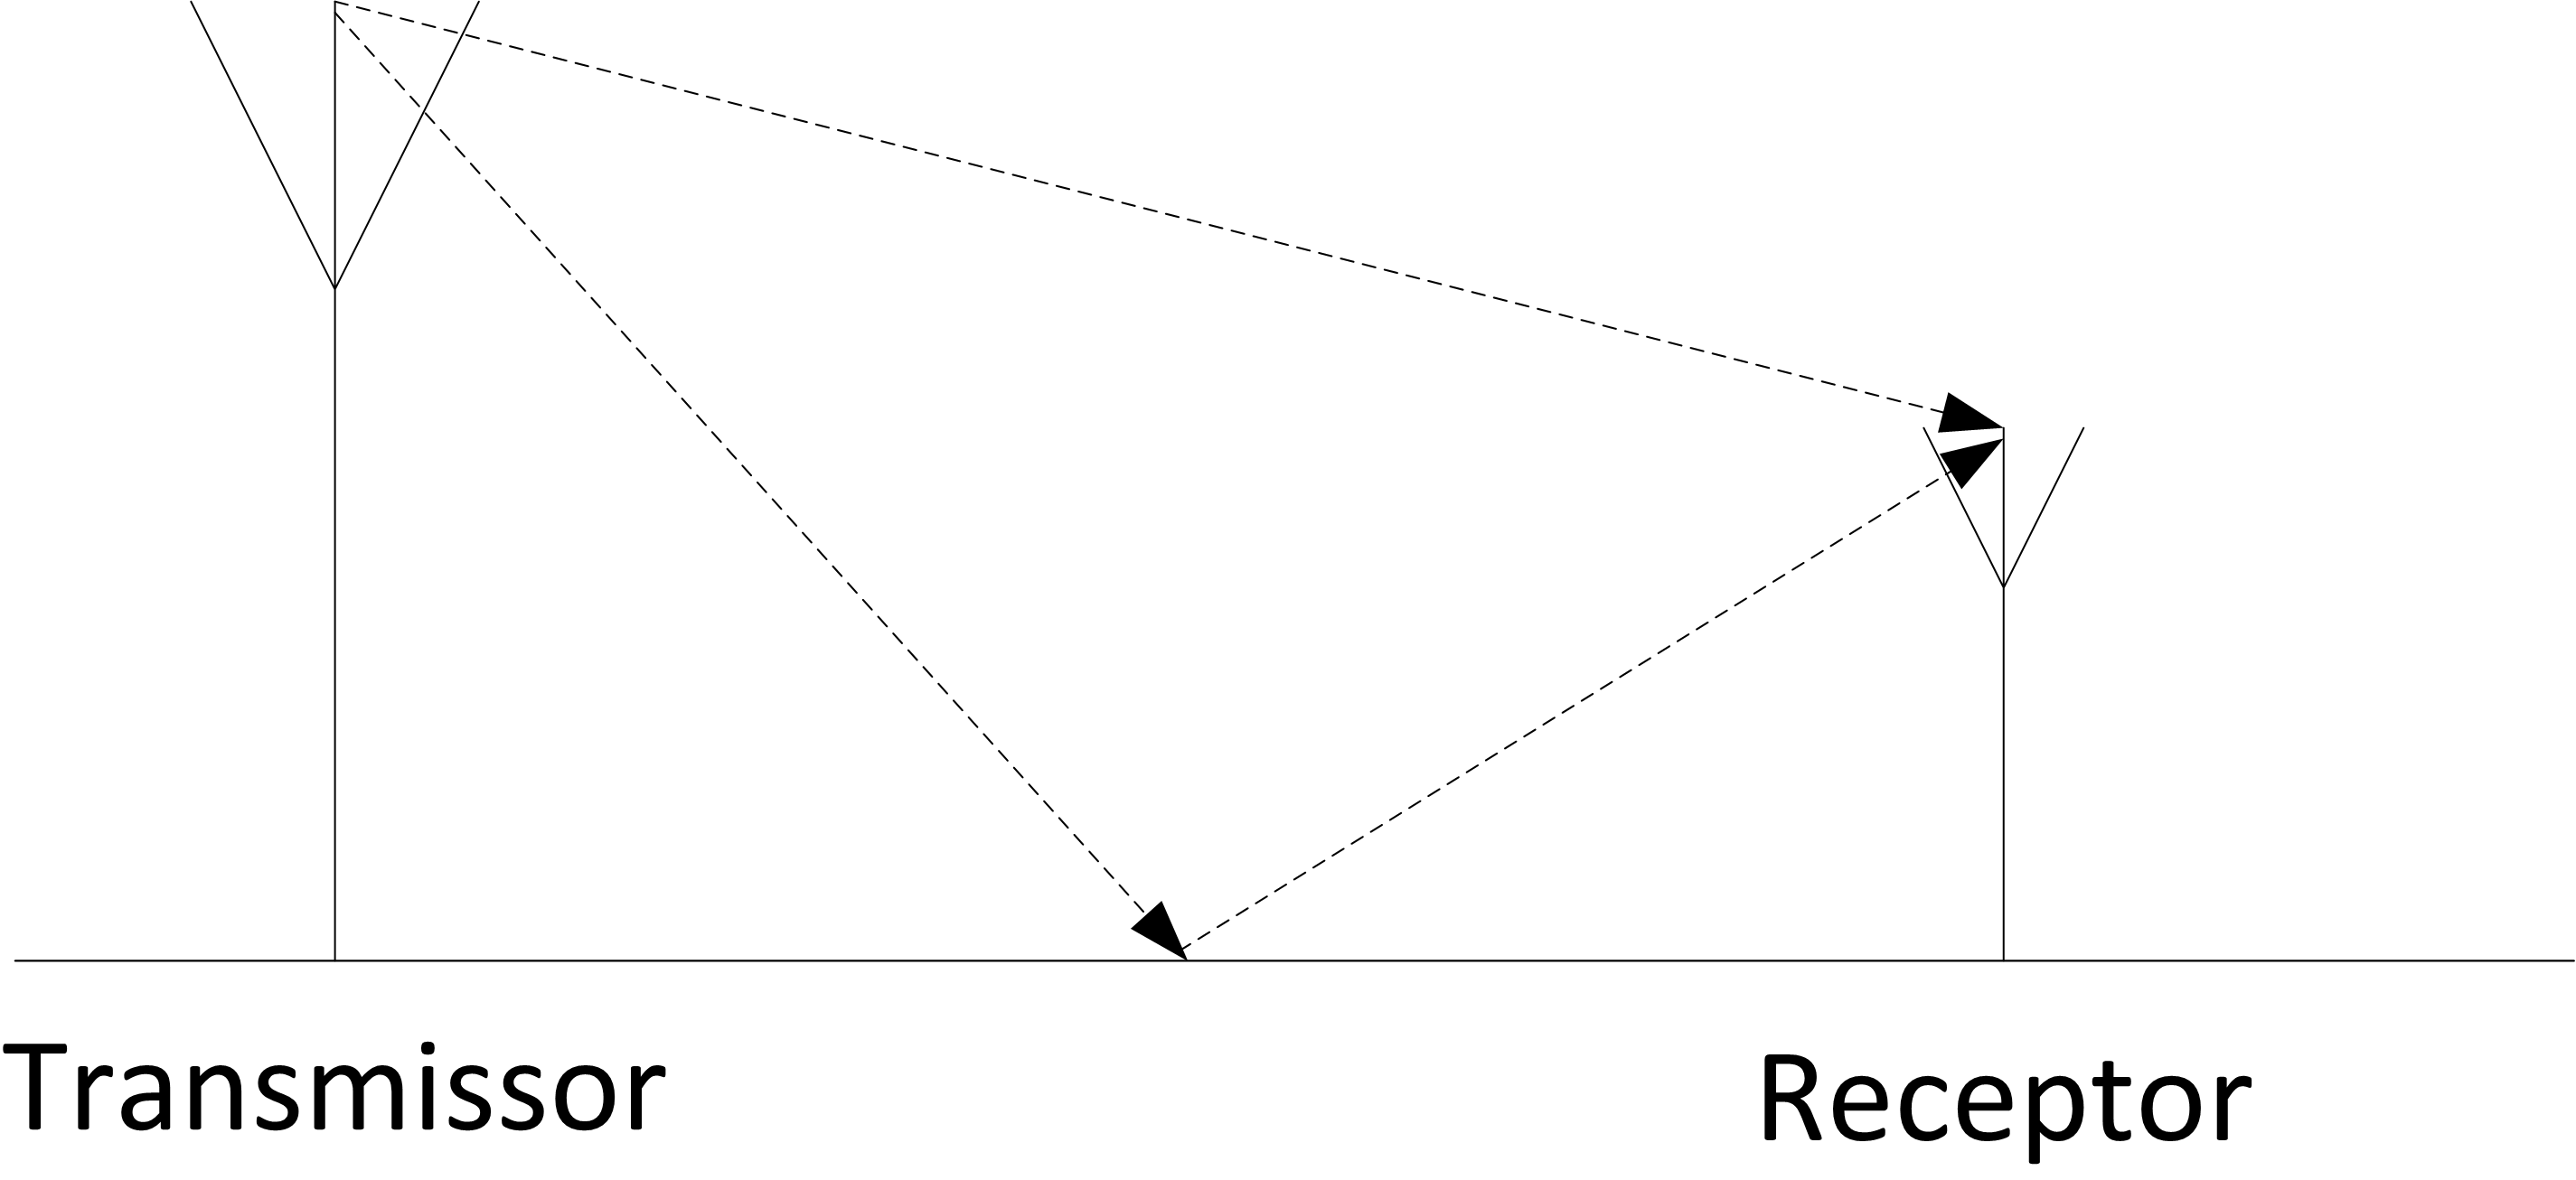
\includegraphics[width=0.8\textwidth]{figs/tworay}
\caption[Modelo de propagação Two Ray Ground.]
{Modelo de propagação Two Ray Ground.}
\label{fig:tworay}
\end{figure}

O modelo Two Ray Ground leva em consideração dois caminhos: O primeiro é equivalente ao Free Spaces, ou seja, um caminho direto do transmissor ao receptor e o segundo é um caminho que incide no solo e é refletido para o receptor. Um exemplo é ilustrado na figura~\ref{fig:tworay}.

A potência recebida pelo receptor quando o transmissor se encontra a uma distância \textit{d} é definida~\cite{rapapport} como: 

\begin{align}
  \label{pottworay} P_r(d) = P_tG_tG_r\frac{h_t^{2}h_r^{2}}{d^4}
\end{align}

Onde \begin{math}h_t\end{math} é a altura da antena transmissora e \begin{math}h_r\end{math} é a altura da antena do receptor em metros. Foi assumida uma altura de 2 metros para casos onde não foi possível determinar a altura do dispositivo.

Assim, assumindo a equação~\ref{ganho}, temos, pelas equações~\ref{pottworay} e~\ref{minPotAnt} o alcance de uma antena no modelo Two Ray Ground:

\begin{align}
  \label{dTwoRayAnt} d_1 = \sqrt[4]{\frac{P_th_t^{2}h_r^{2}}{10kTB}}
\end{align}

De maneira análoga, o alcance de um US pode ser determinado pelas equações~\ref{potfree} e~\ref{minPotDev}:

\begin{align}
  \label{dTwoRayDev} d_2 = \sqrt[4]{\frac{P_th_t^{2}h_r^{2}}{kTB}}
\end{align}


\subsubsection{Log Distance}

O modelo de propagação Log Distance é bastante utilizado para longas distâncias e assume que a potência transmitida por uma antena decai logaritmicamente em relação à distância. Dois fatores principais entram em cena, a perda ocorrida a uma distância muito pequena, e a taxa de decaimento.

\begin{math}L_0\end{math} determina a perda ocorrida a uma distância muito pequena. Foi considerado a distância \begin{math}d_0\end{math} como sendo 1 metro. Essa perda foi calculada no modelo Free Space:

\begin{align}
  \label{L0} L_0 = \left( \frac{4\pi w}{c}\right)^{2}
\end{align}

Onde \begin{math}w\end{math} é o comprimento de onda da freqência utilizada e \begin{math}c\end{math} é a velocidade da luz em metros.

O modelo foi simplificado de forma que o alcance de uma antena é representado por:

\begin{align}
  \label{dLogDistAnt} d_1 = \sqrt[\gamma]{\frac{d_0^{\gamma}10^{\frac{-L_0}{10}}  P_t}{10kTB}}
\end{align}

De maneira análoga, o alcance de um US é representado por:
\begin{align}
  \label{dLogDistDev} d_2 = \sqrt[\gamma]{\frac{d_0^{\gamma}10^{\frac{-L_0}{10}}  P_t}{kTB}}
\end{align}

\begin{math}\gamma \end{math} representa um fator de perda que geralmente recebe valores de 2 a 6. Foi escolhido 3 como sendo valor padrão.

\subsubsection{Constantes}

As seguintes constantes foram assumidas para os cálculos descritos:

\begin{itemize}
\item d =\begin{math}1380\cdot 10^{-23}\end{math}  mW
\item T = 290 K
\item B = 6 MHz
\item c = 299792458 m/s
\end{itemize}

\section{Extensão dos modelos}

Os modelos implementados não levam em conta a perda causada pelo relevo, o que pode gerar resultados menos acurados, podendo causar interferências ou subutilização de canais no espectro. Um novo modelo de propagação foi desenvolvido nesse trabalho, levando em contra outras variáveis para determinar a atenuação do sinal de um dispositivo.

\subsection{Longley-Rice}
\label{subsec:longleyricesection}

Também conhecido como Irregular Terrain Model (ITM)\abbrev{ITM}{Irregular Terrain Model}, este modelo foi proposto para frequências entre 20 MHz a 20GHz, para alturas distintas de antenas transmissoras e receptoras. Dada a frequência, altura das antenas e uma estimativa da irregularidade do terreno, o modelo retorna um valor de referência para a atenuação do sinal. Foi bastante utilizado no auxílio de instalação de redes de telecomunicações, em especial os sistemas de televisão e rádiodifusão na alocação de canais de transmissão Very High Frequency(VHF)
\abbrev{VHF}{Very High Frequency} 
e Ultra High Frequency(UHF)
\abbrev{UHF}{UHF High Frequency}.

Publicado em 1968 por Anita Longley e Phil Rice, esse modelo foi proposto para ser utilizado em um computador e foi criado de forma a abranger diversas combinações de frequências, distâncias, terrenos e climas para ambas polarizações - vertical e horizontal- de uma antena~\cite{longleyrice}.

O Longley-Rice é capaz de predizer a atenuação de dois modos diferentes: o modo área e o modo ponto-a-ponto. O modo área utiliza informações médias de um perfil do terreno para realizar o cálculo da atenuação. Já o modo ponto-a-ponto utiliza informações específicas do caminho entre o transmissor e o receptor para realização o cálculo da atenuação.

\subsubsection{Parâmetros de Entrada}

Para ambos os modos, os parâmetros listados abaixo são necessários:

\begin{itemize}
\item \begin{math}d\end{math} Distância entre os dispositivos
\item \begin{math}k\end{math} Número de onda
\item \begin{math}h_{g1}, h_{g2}\end{math} Altura estrutural das antenas
\item \begin{math}\Delta h\end{math} Parâmetro de irregularidade do terreno
\item \begin{math}N_s\end{math} Refratividade da Superfície
\item \begin{math}\gamma _e\end{math} Curvatura efetiva da terra
\item \begin{math}Z_g\end{math} Impedância da superfície
\item clima Expresso qualitativamente com um número para denotar um tipo de clima discreto
\end{itemize}

Para obtermos o número de onda, basta aplicarmos a fórmula:


\begin{align}
  \label{wn} k = 2\pi/\lambda = f/f_0 \,\,\,\,\, \text{ sendo} \,\,\,\,\,\,\,\,\, f_0 = 47.70 \text{ MHz . m }
\end{align}


O parâmetro de irregularidade do terreno pode ser obtido na tabela~\ref{table:deltah}. \\

\begin{table}[h]
\centering
\caption[Valores para o parâmetro de irregularidade do terreno.]
{Tabela obtida no relatório de Longley, Rice  e Kissick ~\cite{longleyricedelta}} 
\label{table:deltah}
\begin{tabular}{ll}

\hline
                             & $\Delta$ h (metros) \\ \hline
Plano ou sobre a água        & 0                 \\
Planícies                    & 30                \\
Colinas                      & 90                \\
Serras                       & 200               \\
Montanhas                    & 500               
\end{tabular}
\end{table}


O valor do parâmetro de irregularidade varia em função da distância, seguindo a equação abaixo: 
\begin{align}
\label{deltaH} \Delta h(s) = (1-0.8e^{-s/D})\Delta h \,\,\,\, \text{ com $D = 50 $ km e $s$ a distância}
\end{align}

No artigo original do modelo~\cite{longleyrice}, um programa foi apresentado e as previsões da atenuação do sinal foram testadas para um certo intervalo de valores de entrada, onde o modelo provou-se eficiente. Os parâmetros e seus respectivos intervalos estão listados na tabela~\ref{table:longleyricevaluesinterval}:\\

\begin{table}[h]
\centering
\caption[Intervalos válidos para os parâmetros de entrada.]
{Intervalos válidos para os parâmetros de entrada.}
\label{table:longleyricevaluesinterval}
\begin{tabular}{ll}
\hline
Parâmetros                  & Intervalo            \\ \hline
Frequência                  & 20 a 40,000 MHz      \\
Altura das Antenas          & 0.5 a 3,000 m        \\
Distância                   & 1 a 2,000 km         \\
Refratividade da Superfície & 250 a 400 N-unidades
\end{tabular}
\end{table}

A polarização da antena pode ser horizontal ou vertical e afeta o valor da impedância da superfície \begin{math}Z_g\end{math}, ibtida pela análise da permissividad e condutividade do solo em relação à polarização das ondas. A impedância característica do solo em relação a sua polarização é apresentada a seguir:

\[
	      Z_g = \begin{cases} 
	 \sqrt{\epsilon_r' - 1} & \textrm{ Polarização horizontal} \\
       \frac{\sqrt{\epsilon_r' - 1}}{\epsilon_r'} & \textrm{ Polarização vertical} \\
   	\end{cases}
\]

onde \begin{math}\epsilon_r'\end{math} é a Permissividade relativa complexa, definida por:

\begin{align}
\label{eps_r} \epsilon_r' = \epsilon_r + i Z_0\sigma/k
\end{align}
\begin{align}
\label{z_0} Z_0 = 376.62 \textrm{ ohm.}
\end{align}
A condutividade do solo $\sigma$ é expressa em siemens por metro. Seus possíveis valores podem são apresentados na tabela ~\ref{table:sigmainterval}

\begin{table}[h]
\caption[Valores para a permissividade relativa e condutividade do solo.]
{Valores para a permissividade relativa e condutividade do solo.}
\label{table:sigmainterval}
\centering
\resizebox{\textwidth}{!}{%
\begin{tabular}{lcc} \\
\hline
            & Permissividade Relativa & Condutividade (Siemens por metro) \\ \hline
Solo médio  & 15                      & 0.005                             \\
Solo pobre  & 4                       & 0.001                             \\
Solo bom    & 25                      & 0.020                             \\
Água fresca & 81                      & 0.010                             \\
Água do mar & 81                      & 5.0                              
\end{tabular}
}
\end{table}

A curvatura efetiva da terra $\gamma_e$ pode ser obtida através da fórmula:

\begin{align}
\label{ge} \gamma_e = \gamma_a/K
\end{align}


Onde $\gamma_a$ é a curvatura real da terra e $K$ é o fator de raio efetivo da Terra. O valor normalmente é obtido através de sua formúla empírica:
\begin{align}
\label{ge2} \gamma_e = \gamma_a(1-0.04665e^{N_s/N_1})
\end{align}

onde

\begin{align}
\label{n_1} N_1 = 179.3 \text{ N-unidades, e } \gamma_a = 157 . 10^-9 \text{ m} ^-1 = 157 \text{ N-unidades/km.}
\end{align}
A refratividade da superfície \begin{math}N_s\end{math} é obtida a partir da análise das condições atmosféricas, como a temperatura, pressão e umidade relativa. Esse valor determina quantidade de sinal que é refratado pela atmosfera.
Para simplificar a sua representação, a refratividade da superfície  é definida em termos de \begin{math}N_0\end{math}, a refratividade da superfície reduzida ao nível do mar.

\begin{align}
\label{ns} N_s = N_0e^{-z_s/z_1} \,\,\,\,\, \text{ sendo} \,\,\,\,\,\,\,\,\, z_1 = 9.46 \text{ km }
\end{align}
Onde \begin{math}z_s\end{math} é a elevação geral da região envolvida. Para o modo ponto-a-ponto, esse valor é a média aritmética das elevações no caminho entre o transmissor e o receptor.
Ao reduzirmos a refratividade da superfície ao nível do mar, podemos utilizar o mapa presente no relatório ~\cite{longleyricedelta} para obter um valor válido para \begin{math}N_s\end{math}. Os valores são apresentados na figura.~\ref{fig:nsmap} Esses dados podem ser resumidos em função do clima da região em estudo, listados na tabela ~\ref{table:climatetable}.



\begin{table}[h]
\centering
\caption[Refratividade da superfície em função do clima da região.]
{Refratividade da superfície em função do clima da região.}
\label{table:climatetable}
\resizebox{\textwidth}{!}{%
\begin{tabular}{lc}
\hline
Clima                       & Refratividade da superfície (N-unidades) \\ \hline
Deserto                     & 280                                    \\
Continental Temperado       & 301                                    \\
Continental Sub-tropical    & 320                                    \\
Marítimo Temperado          & 320                                    \\
Marítimo temperado sobre o mar & 350                                    \\
Equatorial                  & 360                                    \\
Marítimo Sub-tropical       & 370                                    \\
\end{tabular}
}
\end{table}

\begin{figure}[nsmap]
\centering
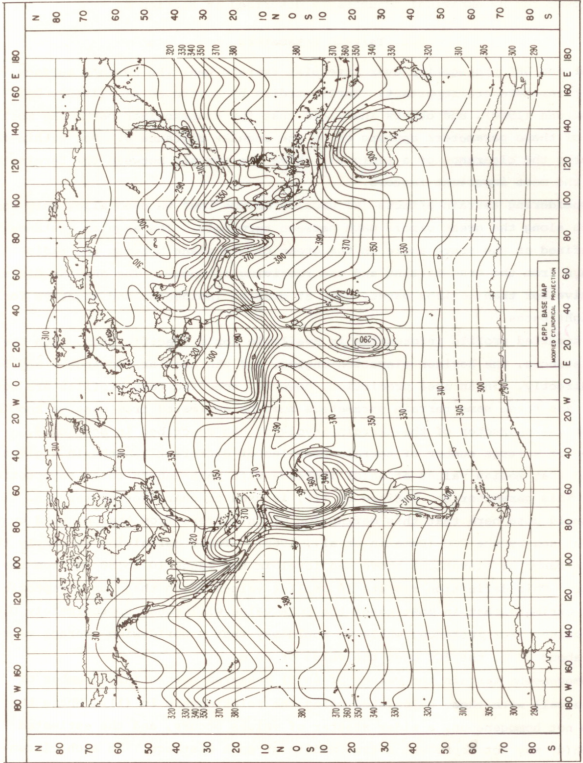
\includegraphics[width=0.8\textwidth]{figs/nsmap}
\caption[Refratividade média da superfície reduzida ao nível do mar.]
{Refratividade média da superfície reduzida ao nível do mar.}
\label{fig:nsmap}
\end{figure}

\subsubsection{Parâmetros adicionais para o modo ponto-a-ponto}

Cada modo depende de diferentes parâmetros de entrada.Nos modo ponto-a-ponto, informações detalhadas do terreno para o caminho entre o transmisso e receptor estão disponíveis, as variáveis adicionais de entrada utilizados pelo algoritmo nesse modo são:

\begin{itemize}
\item \begin{math}h_{e1}, h_{e1}\end{math} Alturas efetivas das antenas
\item \begin{math}d_{L1},d_{L2}\end{math} Distância de cada dispositivo ao seu horizonte
\item \begin{math}\theta_{e1}, \theta_{e2}\end{math} Ângulos de elevação dos horizontes de cada dispositivo na altura das antenas
\end{itemize}

No modo área, esses valores são aproximados utilizando uma fórmula empírica na qual $\Delta h$ influencia fortemente, pois não há informações específicas do caminho a ser percorrido pelas ondas.

A altura efetiva de uma antena é a altura acima de um plano refletor, os valores podem ser encontrados na figura ~\ref{fig:radiohorizon}~\cite{longleyrice}, 

\begin{figure}[radiohorizon]
\centering
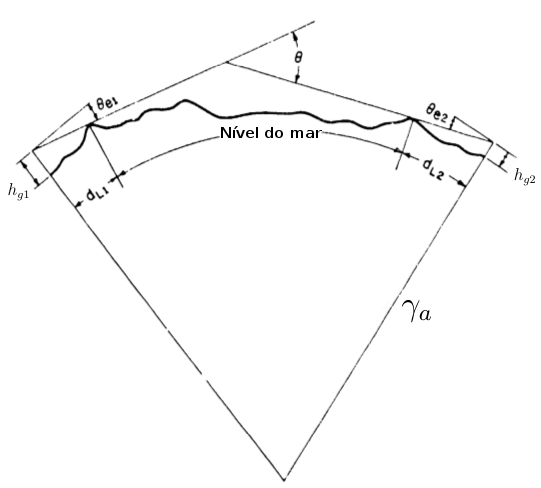
\includegraphics[width=0.8\textwidth]{figs/radiohorizon}
\caption[Geometria de um caminho transhorizonte.]
{Geometria de um caminho transhorizonte.}
\label{fig:radiohorizon}
\end{figure}

O ângulo $\theta$ é obtido da seguinte forma:

\begin{align}
\label{theta} \theta = max(\theta_{e1} + \theta{e2}, -d_{L} \gamma e)
\end{align}

onde

\begin{align}
\label{dl} d_L = d_{L1} + d_L{L2}
\end{align}

\subsubsection{Parâmetros adicionais para o modo área}

O modo área realiza a predição com menos informações sobre o terreno. Portanto, apenas um parâmetro é levado em consideração: o critério de localização do receptor, que pode assumir apenas três valores: Aleatório, com cautela ou com muita cautela.

Os parâmetros \begin{math}h_{ei}, \, d_{Li}, \, \theta_{ei}, \, j=1,2\end{math} não são parâmetos de entrada nesse modo, porque nem sempre as informações específicas do terreno estão disponíveis.No modo área, eles são calculados empiricamente e o critério de localização é utilizado para determinar a altura efetiva da seguinte forma:

\begin{align}
\label{h_ei} h_{ei} = h_{gi} \,\,\,\,\, \text{Se o dipositivo está localizado aleatoriamente}
\end{align}

Se não, assuma que

\[ B_i = \begin{cases} 
      5 \text{ m} & \textrm{ Se o dispositivo está localizado com cautela} \\
      10 \text{ m} & \textrm{ Se o dispositivo está localizado com grande cautela} \\
   \end{cases} \]  
   
e

\[ B'_i = (B_i - H_1)sen(\frac{\pi}{2} min(h_g1/H_2,1)) + H_1 \textrm{, sendo $H_1 = 1$ m, $H_2 = 5$ m} \]

com isso, a altura efetiva é calculada a partir da seguinte equação

\begin{align} 
\label{hei} h_{ei} = h_{gi} + B'_je^{-2h_{gi}/\Delta h}
\end{align}

Em seguida, utilizamos os valores das alturas para determinar $d_{Lsi}\, , i=1,2$, que são as distâncias do horizonte assumindo a Terra como perfeitamente esférica:

\begin{align}
\label{d_lsi} d_{Lsi} = \sqrt{2h_{ei}/\gamma_e}
\end{align}

Com isso, as distâncias do horizonte são obtidas

\begin{align}
\label{d_lj} d_{Lj} = d_{Lsj}e^{-0.07\sqrt{\Delta h / max(h_{ei},H_3)}} \,\,\,\, \text{com $H_3 = 5$ m}
\end{align}

Por fim, os ângulos efetivos $\theta_{ei}, i=1,2$ são calculados através da fórmula:

\begin{align}
\label{oei} 	\theta_{ei} = \frac{0.65\Delta h(d_{Lsi}/d_{Li} -1)}{d_{Lsi}}
\end{align}


\subsubsection{Retorno do algoritmo}

Os parâmetros citados anteriormente são utilizados para computar a perda da transmissão. O resultado é um valor de atenuação calculado através do somatório de duas atenuações: A primeira é utilizando o Free-Spaces citado anteriormente enquanto a segunda é uma atenuação de referência, que pode ser calculada de diferentes maneiras, dependendo da distância entre os dispositivos.

Sejam $A_{lr}$, $A_{fs}$, $A_{ref}$ as atenuações do Longley-Rice, Free Spaces e de referência, respectivamente, o valor da atenuação retornada pelo modelo é:

\begin{align}
\label{a_lr} A_{lr} = A_{fs} + A_{ref}
\end{align}

Para calcular a atenuação (em dB) do Free Spaces, utiliza-se uma fórmula diferente da equação~\ref{potfree}:

\begin{align}
\label{a_fs} A_{fs} = 32.45 + 20 \log_{10}f + 20 \log_{10}d 
\end{align}

Com a frequência $f$ em MHz e a distância $d$ em metros.

\subsubsection{Atenuação de Referência $A_{ref}$}

A atenuação de referência é calculada usando metódos baseados em diferentes modelos de propagação, para três intervalos de distâncias distintas. Na região onde a superfície da terra não interrompe a propagação do sinal, chamada de linha de visada (Line of Sight), o modelo utilizado é o Two Ray, somado ao Free Spaces mencionado anteriormente.

Na região entre $d_{L1}$ e $d_{L2}$, o modelo que prevalece é o de difração\cite{rufford}. Nele, são utilizadas dois modelos para calcular a atenuação: A atenuação de goma dupla de faca e atenuação desenvolvida por Vogler para uma região de difração distante, assumindo a terra perfeitamente esférica~\cite{vogler}.

Quando a distância entre os dispositivos ou $\theta$ é muito grande, calcula-se a atenuação na região de dispersão.

\section{Tecnologias Utilizadas}

O sistema foi desenvolvido utilizando a linguagem de programação orientada a objetos Java, com o Sistema de Gerenciamento de Banco de Dados MYSQL
\abbrev{SGBD}{Sistema de Gerenciamento de Banco de Dados} 
para armazenamento dos dados. O protocolo utilizado para o desenvolvimento da  Application Programming Interface (API)
\abbrev{API}{Application Programming Interface} 
foi o REST, para isso, foi utilizada uma biblioteca Java chamada Restlet~\cite{restlet}. As respostas do sistema são no formato XML ou no formato JSON. O desenvolvimento da base foi realizado no ambiente Eclipse.

A aplicação Web utilizou  HyperText Markup Language(HTML)
\abbrev{HTML}{HyperText Markup Language}
para produção das páginas Web, em conjunto com a linguagem script Javascript para dinamização. Para customizar o layout da página, foi utilizado Cascading Style Sheets(CSS)
\abbrev{CSS}{Cascading Style Sheets}
como linguagem de estilo. Para realização de requisições assíncronas ao servidor, utilizou-se o AJAX. Por fim, para renderização do mapa geográfico na página Web, foi utilizada a API em Javascript de mapas HERE~\cite{heremaps}. 

\section{Banco de Dados}

\subsection{Obtenção dos dados}

Os dados foram obtidos diretamente do site da ANATEL~\cite{channelstable}, de forma manual. Foi baixado um arquivo com as informações de todas as antenas de televisão instaladas no Brasil. No arquivo, estão presentes os seguintes dados:

\begin{itemize}
\item Estado
\item Cidade
\item Dono
\item Tipo
\item Canal
\item Complemento do Canal 
\item Campo Vazio
\item Latitude 
\item Longitude 
\item Potência
\item Informações de Antenas Direcionais
	\subitem Altura
	\subitem Direcionamento
	\subitem Potência
\end{itemize}

Desse arquivo foram extraídas informações das antenas cujo campo $Estado$ era "RJ".

Para identificar qual o canal que uma antena operava, foram utilizados os campos $Canal$ e $Complemento\, do\, Canal$.

Os campos $Latitude$ e $Longitude$ informam a posição da antena no planeta, no formato grau-minuto-segundo, com uma letra indicando a direção da bússola. Essas informações foram convertidas para o formato decimal, para o caso do Estado do Rio de Janeiro, assumiram valores negativos pois o estado está localizado à Oeste e Sul do globo.

O campo \textit{Potência} está em kW e é utilizado como potência da antena.

No arquivo, assume-se que as antenas são multidirecionais, porém, algumas antenas irradiam a uma dada potência apenas em um cone direcionado. Chamadas Antenas Direcionais, essas antenas são descritas no arquivo com os campos \textit{Altura}, \textit{Direcionamento} (em Azimuth) e \textit{Potência}, dentro de \textit{Informações de Antenas Direcionais}.

\subsubsection{Canais de transmissão}

As informações referentes aos canais de transmissão utilizados pelas antenas também foram retiradas do site da ANATEL, e incluídas na base. Na tabela ~\ref{table:tabcanal}, estão as informações de frequência para cada canal.

\begin{center}
\begin{longtable}{cccc}

\caption[Informações sobre os canais de transmissão.]
{Tabela obtida do site da ANATEL}
\label{table:tabcanal} \\

\hline \multicolumn{1}{|c|}{\textbf{Canal}} & \multicolumn{1}{c|}{\textbf{ Frequência Mínima}} & \multicolumn{1}{c|}{\textbf{Frequência Média}}  & \multicolumn{1}{c|}{\textbf{Frequência Máxima}} \\ \hline 
\endfirsthead

\multicolumn{4}{c}%
{{\bfseries \tablename\ \thetable{} -- continuação}} \\
\hline 
\multicolumn{1}{|c|}{\textbf{Canal}} &
\multicolumn{1}{c|}{\textbf{Frequência Mínima}} &
\multicolumn{1}{c|}{\textbf{Frequência Média }} &
\multicolumn{1}{c|}{\textbf{Frequência Máxima}} \\ \hline 
\endhead

\hline 
\endfoot

\hline \hline
\endlastfoot

2 & 54 & 57 & 60 \\ 
3 & 60 & 63 & 66 \\ 
4 & 66 & 69 & 72 \\ 
5 & 76 & 79 & 82 \\ 
6 & 82 & 85 & 88 \\ 
7 & 174 & 177 & 180 \\ 
8 & 180 & 183 & 186 \\ 
9 & 186 & 189 & 192 \\ 
10 & 192 & 195 & 198 \\ 
11 & 198 & 201 & 204 \\ 
12 & 204 & 207 & 210 \\ 
13 & 210 & 213 & 216 \\ 
14 & 470 & 473 & 476 \\ 
15 & 476 & 479 & 482 \\ 
16 & 482 & 485 & 488 \\ 
17 & 488 & 491 & 494 \\ 
18 & 494 & 497 & 500 \\ 
19 & 500 & 503 & 506 \\ 
20 & 506 & 509 & 512 \\ 
21 & 512 & 515 & 518 \\ 
22 & 518 & 521 & 524 \\ 
23 & 524 & 527 & 530 \\ 
24 & 530 & 533 & 536 \\ 
25 & 536 & 539 & 542 \\ 
26 & 542 & 545 & 548 \\ 
27 & 548 & 551 & 554 \\ 
28 & 554 & 557 & 560 \\ 
29 & 560 & 563 & 566 \\ 
30 & 566 & 569 & 572 \\ 
31 & 572 & 575 & 578 \\ 
32 & 578 & 581 & 584 \\ 
33 & 584 & 587 & 590 \\ 
34 & 590 & 593 & 596 \\ 
35 & 596 & 599 & 602 \\ 
36 & 602 & 605 & 608 \\ 
38 & 614 & 617 & 620 \\ 
39 & 620 & 623 & 626 \\ 
40 & 626 & 629 & 632 \\ 
41 & 632 & 635 & 638 \\ 
42 & 638 & 641 & 644 \\ 
43 & 644 & 647 & 650 \\ 
44 & 650 & 653 & 656 \\ 
45 & 656 & 659 & 662 \\ 
46 & 662 & 665 & 668 \\ 
47 & 668 & 671 & 674 \\ 
48 & 674 & 677 & 680 \\ 
49 & 680 & 683 & 686 \\ 
50 & 686 & 689 & 692 \\ 
51 & 692 & 695 & 698 \\ 
52 & 698 & 701 & 704 \\ 
53 & 704 & 707 & 710 \\ 
54 & 710 & 713 & 716 \\ 
55 & 716 & 719 & 722 \\ 
56 & 722 & 725 & 728 \\ 
57 & 728 & 731 & 734 \\ 
58 & 734 & 737 & 740 \\ 
59 & 740 & 743 & 746 \\ 
60 & 746 & 749 & 752 \\ 
61 & 752 & 755 & 758 \\ 
62 & 758 & 761 & 764 \\ 
63 & 764 & 767 & 770 \\ 
64 & 770 & 773 & 776 \\ 
65 & 776 & 779 & 782 \\ 
66 & 782 & 785 & 788 \\ 
67 & 788 & 791 & 794 \\ 
68 & 794 & 797 & 800 \\ 
69 & 800 & 803 & 806 \\ 

\end{longtable}
\end{center}


\subsection{Confiabilidade dos Dados}

Para o funcionamento apropriado da base, os dados oriundos da ANATEL devem ser consistentes. No entando, após análise dos mesmo, nota-se que o arquivo possui diversos erros. Algumas antenas estão localizadas em São Paulo, porém o campo \textit{Estado} possui valor "RJ". Além disso, no campo \textit{Elevação}, utilizado para definir a altura de determinada antena, possuía valores muito grandes, acima de 1.5km e valores abaixo de zero, o que é impossível fisicamente.
Outro problema é a pouca precisão nos valores de \textit{Latitude} e \textit{Longitude} das antenas.

Essa ausência de confiabilidade acaba prejudicando os modelos de propagação do sinal da antena, portanto é necessária uma cooperação com a ANATEL para melhorar a qualidade desses dados.

\subsection{Base de Dados}

A partir do arquivo da ANATEL, foi modelado um banco de dados que armazenasse as informações das antenas, dos canais e foram criados três tipos diferentes de USs.

Para os USs, foram criados três tipos de dispositivos:

\begin{table}[h]
\centering
\caption[Tipos de dispositivos para Usuários Secundários.]
{Tipos de dispositivos para Usuários Secundários.} 
\label{table:wstypes}
\begin{tabular}{lc}

\hline
Tipo de Dispositivo          & Potência (mW)     \\ \hline
INTERNO BAIXO                & 10                \\
INTERNO ALTO                 & 50                \\
EXTERNO                      & 100                     
\end{tabular}
\end{table}

São três classes de dispositivos com potências pré-definidas. Se o dispositivo for utilizado dentro de alguma construção, será do tipo "INTERNO", enquanto dispositivos de uso externo, no tipo "EXTERNO".

Com essas informações, foram implementadas cinco tabelas no banco.

Na tabela Channels, temos informações sobre o número do canal e as frequências mínima, média e máxima de transmissão nesse canal.

As tabelas \textit{Antenas} e \textit{Ws\_Devices} apontam para um determinado canal, através da coluna \textit{channel\_id} e dentro de ambas as tabelas temos a sua localização.

Nas \textit{Antenas}, existem informações da sua potência e elevação. Foi criada também uma tabela para antenas direcionais a \textit{Directed\_Antenas}.

Na tabela de dispositivos secundários, \textit{Ws\_Devices}, existe uma coluna que referencia o tipo de dispositivo \textit{device\_class\_id}. Os tipos de dispositivos são armazenados em uma tabela separada, denominada \textit{Device\_Class}.

O design do banco de dados pode ser observado na figura ~\ref{fig:databasebefore}.


\begin{figure}[databasebefore]
\centering
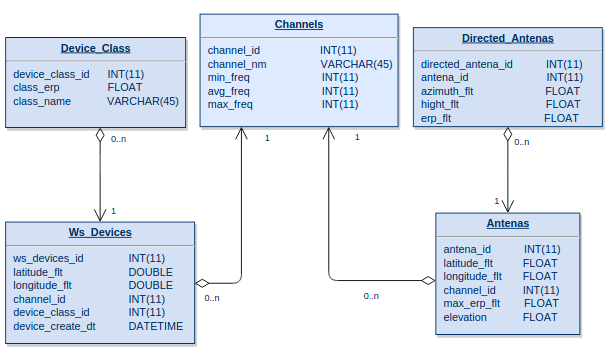
\includegraphics[width=1.0\textwidth]{figs/databasebefore}
\caption[Estrutura da base de dados.]
{Estrutura da base de dados.}
\label{fig:databasebefore}
\end{figure}


\section{Web Service}

Como citado na seção anterior, o servidor realiza a consulta ao banco de dados e obtém as informações dos UPs, em seguida aplica um dos modelos de propagação implementados e retorna uma lista com os canais livres baseada na posição geográfica do US.

\subsection{REST}
\textit{Representational State Transfer(REST)} é um padrão de arquitetura de software. Consiste em diretrizes para criação de \textit{Web Services} escaláveis e é amplamente utilizado na Web, por ser uma alternativa mais simples ao \textit{Simple Object Access Protocol (SOAP)} e \textit{Web Services Description Language (WSDL)},
 criado em 2000, na tese doutorado de Roy T. Fielding ~\cite{restcreator}.
 
Além de simplificar as interfaces, esse padrão é performático e escalável.

Sistemas REST tipicamente utilizam o protocolo HTTP com os mesmos métodos (GET,POST,PUT E DELETE) utilizado pelos browsers para carregar páginas e enviar dados à servidores.

Ele assume que a base consiste de recursos, que podem ser acessados via URL. Cada recurso tem seu próprio identificador, denominado \textit{Unified Resource Identifier}(URI).

\abbrev{URI}{Uniform Resource Identifier}

Esse recursos, por sua vez, são acessados por requisições HTTP, divididos em quatro tipos citados anteriormente:

\begin{itemize}
\item GET - realiza a busca de um recurso
\item POST - utilizado para alterar o valor de um recurso
\item PUT - utilizado para alterar o valor de um recurso
\item DELETE - utilizado para excluir um recurso
\end{itemize}

O POST e o PUT são bastante semelhantes, mas segundo a especificação do HTTP ~\cite{RFC2616}, o método POST deve ser utilizado na criação de um novo recurso, enquanto o PUT somente para a alteração de recursos criados anteriormente. No entando, o POST também é utilizado para alteração de recursos já existentes na base e foi utilizado dessa forma também no desenvolvimento do Web Service deste trabalho.

Não existe uma forma padrão para a resposta do servidor ao cliente. Entretanto, isso muitas vezes é feito via JSON ou XML, já que estes formatos apresentam uma forma mais estruturada. No servidor desenvolvido o formato de resposta escolhido foi o XML e posteriormente algumas respostas foram modificadas para JSON, visando uma melhor comunicação com a interface Web.

\begin{figure}[clientserver]
\centering
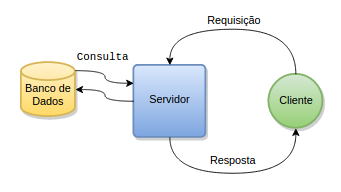
\includegraphics[width=1.0\textwidth]{figs/clientserver}
\caption[Arquitetura cliente servidor.]
{Arquitetura cliente servidor.}
\label{fig:clientserver}
\end{figure}


Um possível fluxo de uma requisição pode ser seguinte maneira:

\begin{itemize}
\item O cliente faz um pedido HTTP através de uma URL ao servidor
\item Baseado na URI da URL, o servidor localiza o recurso no banco
\item O servidor processa o pedido e retorna o recurso
\item O cliente recebe a resposta do servidor no formato XML ou JSON
\end{itemize}


\subsection{Classes}
A linguagem utilizada para a implemetanção do servidor foi Java, uma linguagem orientada a objetos onde todos os arquivos são classes. O padrão de desenvolvimento adotado por Machado~\cite{tccmarcelo} foi o de Fábricas.

Esse padrão de desenvolvimento consiste em definir interfaces nas quais os objetos devem estender. Existem também objetos Fábrica, que são responsáveis pela instanciação dos objetos que implementam as interfaces citadas anteriormente. Dessa forma, nenhum objeto é referenciado diretamente.

As classes \textit{Factories} implementadas são representadas na figura abaixo~\ref{fig:facto}

\begin{figure}[htb]
\centering
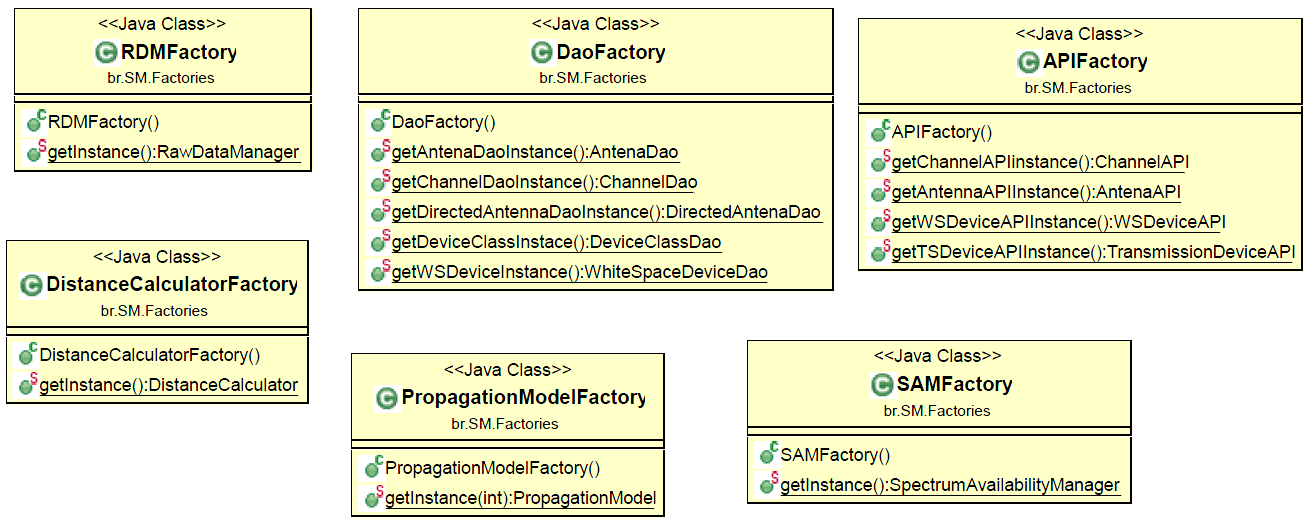
\includegraphics[width=1.0\textwidth]{figs/factories}
\caption[\textit{Factories}.]
{Diagrama de classe das - \textit{Factories}~\cite{tccmarcelo} }
\label{fig:facto}
\end{figure} 


Cada fábrica é responsável por instanciar um componente que será utilizado no servidor. 

A fábrica \textit{PropagationModelFactory} possui um método chamado \textit{getModelInstance()}, que recebe como parâmetro de entrada um inteiro referente ao modelo de propagação desejado. Os modelos estão mapeados no servidor conforme a tabela ~\ref{table:modelnumbers}.

O último modelo não foi implementado na versão inicial do servidor, sendo implementada nesse trabalho. O modelo é explicado na seção ~\ref{subsec:longleyricesection}.

\begin{table}[modelnumbers]
\centering
\caption[Código dos modelos de Propagação no Servidor.]
{Código dos modelos de Propagação no Servidor.} 
\label{table:modelnumbers}
\begin{tabular}{lc}
Modelo de Propagação          & Valor            \\ \hline
Free Spaces                   & 0                \\
Log Distance                  & 1                \\
Two Ray Ground                & 2                \\
Longley-Rice                  & 3                        
\end{tabular}
\end{table}

A \textit{DaoFactory} é a fábrica responsável pela comunicação com o banco de dados. Cada objeto que ela instancia está relacionado à uma tabela do banco.

A \textit{APIFactory} é responsável pelo mapeamento das requisições oriundas do Cliente em métodos do servidor e retorna a resposta no formato JSON ou XML.

A \textit{DistanceCalculatorFactory} é responsável pelo cálculo das distâncias entre os pontos no globo, essa classe é importante para determinar se há interferência ou não, conforme demonstrado na equação ~\ref{cantransmitdata}.

As Fábricas citadas acima foram modificadas para implementação do novo algoritmo e suas alterações são especificadas no próximo capítulo.

\subsection{API}

A comunicação com o servidor é realizada via API, onde uma URL é enviada através de um dos métodos HTTP citados anteriormente. A seguir, a lista das possíveis URLs implementadas no projeto de Machado~\cite{tccmarcelo}. 

\begin{itemize}
\item http://servidor/SAM/devices
\begin{itemize}
	\item GET -- Busca todos os dispositivos de transmissão presentes na base;
\end{itemize}
\item http://servidor/SAM/devices/location
\begin{itemize}
	\item GET -- Busca todos os dispositivos de transmissão presentes na base dada uma localização;
\end{itemize}
\item http://servidor/SAM/devices/channel
\begin{itemize}
	\item GET -- Busca todos os dispositivos de transmissão presentes na base dado um canal;
\end{itemize}
\item http://servidor/SAM/devices/antennas
\begin{itemize}
	\item GET -- Busca todas as antenas presentes na base;
\end{itemize}
\item http://servidor/SAM/devices/antennas/location
\begin{itemize}
	\item GET -- Busca todas as antenas presentes na base dada uma localização;
\end{itemize}
\item http://servidor/SAM/devices/antennas/channel
\begin{itemize}
	\item GET -- Busca todas as antenas presentes na base dado um canal;
\end{itemize}
\item http://servidor/SAM/devices/ws
\begin{itemize}
	\item GET -- Busca todos os dispositivos secundários presentes na base;
	\item PUT -- Cadastra um dispositivo secundário na base;
	\item DELETE -- Remove um dispositivo secundário na base;
\end{itemize}
\item http://servidor/SAM/devices/ws/location
\begin{itemize}
	\item GET -- Busca todos os dispositivos secundários na base dada uma localização;
\end{itemize}
\item http://servidor/SAM/devices/ws/channel
\begin{itemize}
	\item GET -- Busca todos os dispositivos secundários na base dado um canal;
\end{itemize}
\item http://servidor/SAM/devices/ws/classes
\begin{itemize}
	\item GET -- Busca todos os tipos de dispositivos secundários cadastrados na base;
\end{itemize}
\item http://servidor/SAM/channels
\begin{itemize}
	\item GET -- Busca todos os canais cadastrados na base;
\end{itemize}
\item http://servidor/SAM/channels/available
\begin{itemize}
	\item GET -- Busca os canais disponíveis para uso por um determinado dispositivo;
\end{itemize}
\end{itemize}

Uma descrição mais detalhada do funcionamento da API e as classes relacionadas, parâmetros de entrada e o formato da resposta do servidor pode ser encontrada na tese de Machado ~\cite{tccmarcelo}.
